\documentclass[11pt]{article}
\usepackage[T1]{fontenc}
\usepackage{newtxtext,newtxmath}
\usepackage[margin=1in]{geometry}
\usepackage{amsmath}
\usepackage{booktabs}
\usepackage{siunitx}
\usepackage{graphicx}
\usepackage{pgfplots}
\pgfplotsset{compat=1.18}
\pgfplotsset{table/col sep=comma}
\usepackage{xcolor}
\usepackage{caption}
\usepackage{subcaption}
\usepackage{enumitem}
\usepackage{tcolorbox}
\usepackage{microtype}
\usepackage[hidelinks]{hyperref}
\usepackage{xurl}

\definecolor{inkblue}{HTML}{1F4E79}
\definecolor{inkorange}{HTML}{C55A11}
\definecolor{inkteal}{HTML}{2F7D6D}
\definecolor{inkgray}{HTML}{7F7F7F}

\sisetup{detect-all}
\newcommand{\N}{\mathcal{N}}
\newcommand{\E}{\mathbb{E}}
\newcommand{\Q}{\mathbb{Q}}
\newcommand{\R}{\mathbb{R}}
\newcommand{\dd}{\mathrm{d}}
\newcommand{\PV}{\operatorname{PV}}
\newcommand{\ind}[1]{\mathbf{1}_{\{#1\}}}

\title{\bfseries Fair Value of a Bitcoin Dual-Investment Note\\[2pt]
\large Theory and a Live Cross-Section from Binance}
\author{Quantitative research note}
\date{20 October 2026 (CST) \\ \small Data snapshot: 19 October 2026, 16:10 UTC}

\begin{document}

\maketitle

\begin{abstract}
\noindent
A one-unit claim pays $e^{\theta(T-t)}[(S_T/K)\ind{S_T<K}+\ind{S_T\ge K}]$ at $T$, where $S$ is a geometric Brownian motion. We show that the fair continuously compounded $\theta$ is available in closed form,
\[
\theta^\star=-\frac{1}{\tau}\log V_0,\qquad
V_0=\frac{S_t}{K}\N(-d_1)+e^{-r\tau}\N(d_2),\qquad \tau=T-t,
\]
and is independent of the real-world drift $\mu$. We then identify the contract with Binance's \emph{Dual Investment} ``Buy Low'' product, pull the complete live BTC/USDT book (383 strike--tenor combinations, 19 settlement dates) and Binance's own option-implied surface, and compare. At the option-implied surface every one of the 383 quotes has a present value below the 1 unit invested; the median gap is \SI{0.91}{\percent} of principal for maturities of two days or more, rising to about \SI{5}{\percent} at five months. The quotes are consistent with a pricing volatility of \SI{20}{\percent}--\SI{27}{\percent}, against a median of \SI{38.7}{\percent} in listed options. The difference is the price of the desk's short-volatility position, not a free lunch. A near-money two-day note advertising a \SI{94.9}{\percent} APR pays only \SI{0.52}{\percent} flat and loses \SI{1.6}{\percent} if Bitcoin falls \SI{2.4}{\percent}.
\end{abstract}

\begin{tcolorbox}[colback=inkblue!4,colframe=inkblue!55,title=\textbf{Key numbers at the snapshot}]
\begin{itemize}[leftmargin=1.2em,itemsep=2pt,topsep=2pt]
\item Spot BTC/USDT: \num{81990.33}; 383 Buy Low products; tenors \num{0.66}--\num{157.7} days; quoted APRs \SI{3.68}{\percent}--\SI{94.94}{\percent}.
\item Median present value of 1 USDT invested: \num{0.991} (median cost \SI{0.91}{\percent}); maximum cost \SI{4.96}{\percent}; all 383 quotes below the option-implied value.
\item Median quoted APR as a fraction of the option-implied fair APR: \num{0.47}.
\item Median implied pricing volatility: \SI{24.9}{\percent}, versus \SI{38.7}{\percent} median listed implied volatility at the same strikes.
\item 69 quotes (\SI{18}{\percent}) pay less than the risk-free rate embedded in Binance's option marks for the same expiry.
\end{itemize}
\end{tcolorbox}

\section{The contract and the pricing problem}

Let $(\Omega,\mathcal{F},(\mathcal{F}_t)_{t\ge0},\Q)$ be a filtered probability space carrying a standard Brownian motion $B$. Under the risk-neutral measure $\Q$ the Bitcoin price follows
\begin{equation}\label{eq:gbm}
\dd S_t=r S_t\,\dd t+\sigma S_t\,\dd B_t,
\qquad
S_T=S_t\exp\!\left[\left(r-\tfrac12\sigma^2\right)\tau+\sigma\sqrt{\tau}\,Z\right],
\end{equation}
with $\tau=T-t$, $Z\sim\N(0,1)$, constant $r$ and $\sigma>0$. Bitcoin pays no dividend; we treat the USDT rate $r$ as the carry and discount rate. The real-world drift $\mu$ in the question does not appear in \eqref{eq:gbm}: under $\Q$ it is replaced by $r$. This is the first substantive point---the fair value of the note is independent of any view on $\mu$.

The note is bought at $t$ for one unit of account and pays, at $T$,
\begin{equation}\label{eq:payoff}
X_T=e^{\theta(T-t)}\left[\frac{S_T}{K}\ind{S_T<K}+\ind{S_T\ge K}\right].
\end{equation}
The bracket is the normalized payoff $g(S_T)$: in the down state the note delivers $1/K$ units of Bitcoin, worth $S_T/K$ USDT; in the up state it delivers one unit of cash. The factor $e^{\theta\tau}$ is the gross return, paid on \emph{both} branches. This is exactly Binance's Buy Low settlement with $e^{\theta\tau}=1+R$, where $R$ is the flat reward. ``Fair'' means that the arbitrage-free value at $t$ equals the 1 unit paid:
\begin{equation}\label{eq:fair}
\PV(\theta):=\E^{\Q}\!\left[e^{-r\tau}X_T\right]=1.
\end{equation}

\begin{tcolorbox}[colback=inkgray!6,colframe=inkgray!55,title=\textbf{A note on the displayed formula}]
The bracket must \emph{multiply} the exponential, not sit inside it. If the payoff is read literally as $X_T=\exp\{\theta\tau\,g(S_T)\}$, the down state pays $e^{\theta\tau S_T/K}$, which is convex in $S_T$ and is not Binance's linear settlement $(1+R)S_T/K$; the up state pays $e^{\theta\tau}$. The form \eqref{eq:payoff} is the one that matches the live product. The literal exponential-of-payoff reading is discussed in Appendix~\ref{app:literal}.
\end{tcolorbox}

\section{Closed-form fair \texorpdfstring{$\theta$}{theta}}

Let $d_1,d_2$ be the Black--Scholes terms
\begin{equation}\label{eq:d1d2}
d_1=\frac{\log(S_t/K)+(r+\tfrac12\sigma^2)\tau}{\sigma\sqrt{\tau}},
\qquad
d_2=d_1-\sigma\sqrt{\tau}.
\end{equation}
Two standard facts are used. First,
\begin{equation}\label{eq:probs}
\Q(S_T<K)=\N(-d_2),\qquad \Q(S_T\ge K)=\N(d_2).
\end{equation}
Second, the asset-or-nothing expectation is
\begin{equation}\label{eq:asset}
\E^{\Q}\!\left[S_T\ind{S_T<K}\right]=S_t e^{r\tau}\N(-d_1).
\end{equation}
Substituting \eqref{eq:asset} and \eqref{eq:probs} into \eqref{eq:fair},
\begin{align}
\PV(\theta)
&=e^{-r\tau}e^{\theta\tau}\left[\frac{1}{K}S_t e^{r\tau}\N(-d_1)+\N(d_2)\right] \notag\\
&=e^{\theta\tau}\left[\frac{S_t}{K}\N(-d_1)+e^{-r\tau}\N(d_2)\right]
=e^{\theta\tau}V_0.
\label{eq:pvtheta}
\end{align}
Setting $\PV(\theta)=1$ and solving gives the main result.

\begin{tcolorbox}[colback=inkblue!4,colframe=inkblue!60,title=\textbf{Proposition 1 (fair \texorpdfstring{$\theta$}{theta})}]
For the contract \eqref{eq:payoff}, the unique fair rate is
\begin{equation}\label{eq:thetastar}
\boxed{\;\theta^\star=-\frac{1}{\tau}\log V_0
=-\frac{1}{\tau}\log\left[\frac{S_t}{K}\N(-d_1)+e^{-r\tau}\N(d_2)\right]\;}
\end{equation}
with $d_1,d_2$ as in \eqref{eq:d1d2}. The value \eqref{eq:pvtheta} is strictly increasing in $\theta$, so the solution is unique. $\theta^\star$ depends on $S_t/K$, $\tau$, $\sigma$ and $r$, but not on $\mu$.
\end{tcolorbox}

\noindent
Equation \eqref{eq:thetastar} is the answer to the pricing question. Three features are worth isolating.

\begin{enumerate}[leftmargin=1.4em,itemsep=3pt]
\item \textbf{The drift is irrelevant.} A higher $\mu$ raises the physical probability of the up state, but it also raises the discount rate applied to that state; under $\Q$ the two effects cancel exactly. Any claim that the fair $\theta$ ``should'' be higher because Bitcoin is expected to rise is a statement about the physical measure, not about fair value.

\item \textbf{The moneyness is leveraged.} The fair rate is driven by $V_0$, the value of the normalized payoff. A lower strike raises $V_0$ and lowers $\theta^\star$: at two days, moving $K/S_t$ from $1.000$ to $0.997$ cuts the fair rate from \SI{165}{\percent} to \SI{139}{\percent}. At $K=S_t$ and small $\tau$, $V_0\approx1-\tfrac12 r\tau-\phi(0)\sigma\sqrt{\tau}$, so
\begin{equation}\label{eq:atmapprox}
\theta^\star\approx \frac{r}{2}+\frac{\phi(0)\sigma}{\sqrt{\tau}}
=\frac{r}{2}+\frac{0.3989\,\sigma}{\sqrt{\tau}},
\end{equation}
where $\phi(0)=1/\sqrt{2\pi}$. The $1/\sqrt{\tau}$ scaling is the reason short-dated notes carry very large fair APRs: the short put embedded in the normalized payoff has a time value proportional to $\sigma\sqrt{\tau}$, but that value is earned over a period of length $\tau$, so the annualized compensation scales as $\sigma/\sqrt{\tau}$.

\item \textbf{The fair rate can be enormous.} For $\sigma=\SI{30}{\percent}$, $r=\SI{5.3}{\percent}$ and $K=S_t$, \eqref{eq:atmapprox} gives $\theta^\star\approx\SI{232}{\percent}$ at one day, \SI{165}{\percent} at two days, \SI{90}{\percent} at one week and \SI{45}{\percent} at one month; the exact value at one year is \SI{15.5}{\percent}. These are not expected returns; they are the gross return required to compensate the short put. A \SI{30}{\percent} APR on a two-day near-money note is not ``high'' in this metric---it is roughly one-fifth of the fair rate.
\end{enumerate}

Table~\ref{tab:theta} evaluates \eqref{eq:thetastar} across strike ratios and tenors, and Figure~\ref{fig:payoff} shows the two branches. Figure~\ref{fig:theta-sigma} shows the dependence on $\sigma$: near the money the fair rate rises with volatility, because the embedded put becomes more valuable.

\begin{table}[t]
\centering
\caption{Fair continuously compounded rate $\theta^\star$ (percent per annum) for the contract \eqref{eq:payoff}, with $r=\SI{5.3}{\percent}$ and $\sigma=\SI{30}{\percent}$. Columns are tenor in days; rows are $K/S_t$. The at-the-money column follows the $1/\sqrt{\tau}$ law \eqref{eq:atmapprox}.}
\label{tab:theta}
\begin{tabular}{lrrrrrr}
\toprule
$K/S_t$ & 1 d & 2 d & 7 d & 30 d & 90 d & 365 d\\
\midrule
1.000 & 232 & 165 & 90 & 45 & 28 & 16\\
0.997 & 182 & 139 & 82 & 43 & 27 & 15\\
0.994 & 140 & 117 & 75 & 42 & 26 & 15\\
0.990 & 95 & 90 & 67 & 40 & 26 & 15\\
0.980 & 32 & 45 & 48 & 34 & 24 & 15\\
\bottomrule
\end{tabular}
\end{table}

\begin{figure}[t]
\centering
\begin{subfigure}[t]{0.47\textwidth}
\centering
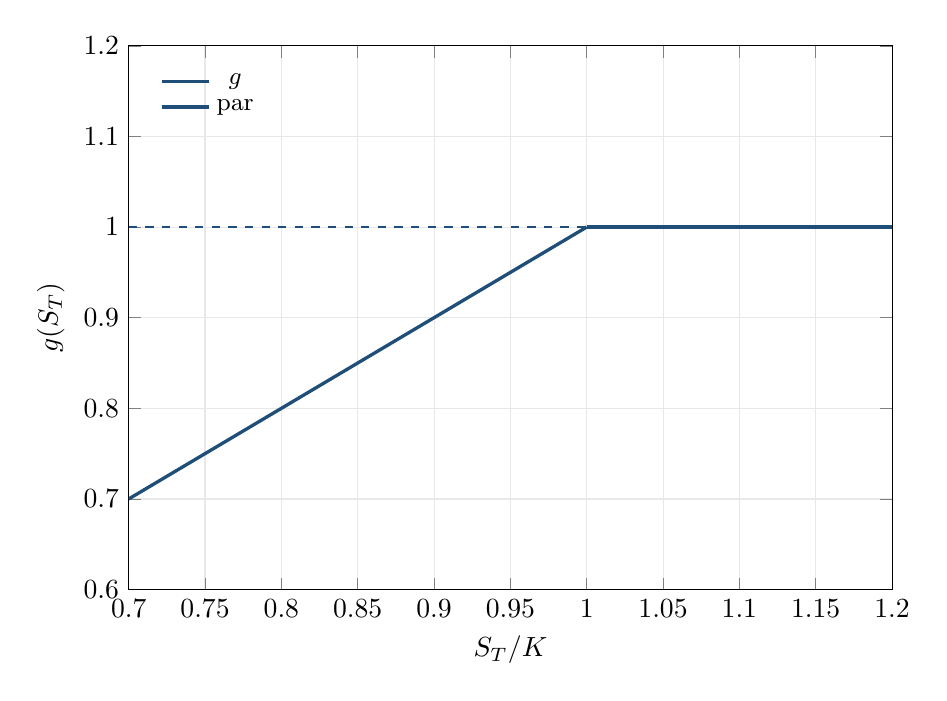
\begin{tikzpicture}
\begin{axis}[width=0.93\linewidth,height=0.70\linewidth,
  xlabel={$S_T/K$},ylabel={$g(S_T)$},
  xmin=0.7,xmax=1.2,ymin=0.6,ymax=1.2,
  grid=major,grid style={gray!18},
  legend pos=north west,legend style={font=\small,draw=none,fill=none}]
\addplot[inkblue,very thick,domain=0.7:1.0,samples=120] {x};
\addplot[inkblue,very thick,domain=1.0:1.2,samples=2] {1};
\addplot[inkblue,dashed,thick,domain=0.7:1.2,samples=2] {1};
\legend{$g$, par}
\end{axis}
\end{tikzpicture}
\caption{Normalized payoff}
\end{subfigure}\hfill
\begin{subfigure}[t]{0.47\textwidth}
\centering
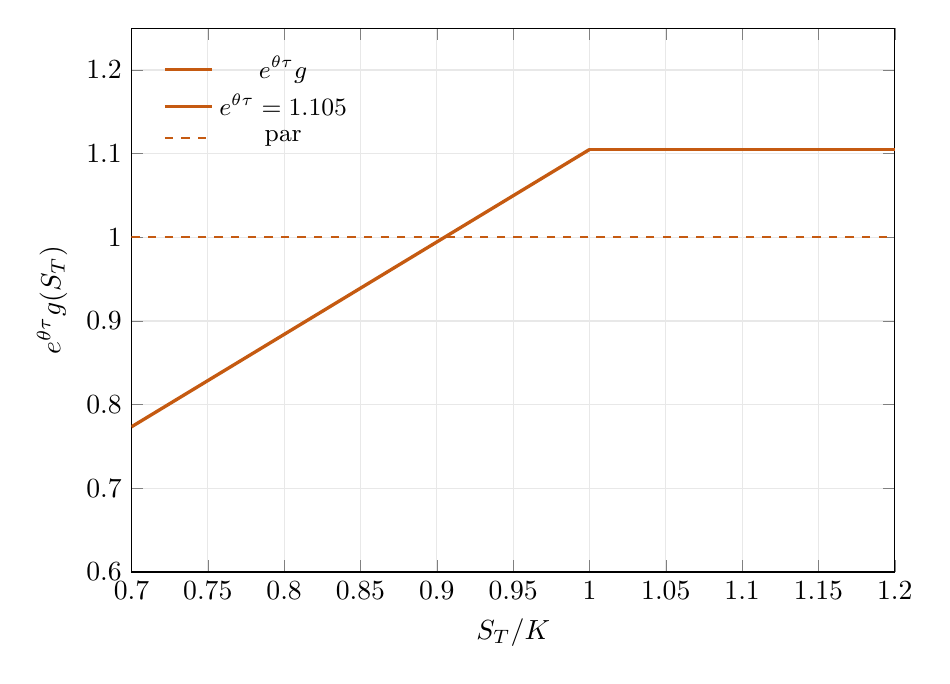
\begin{tikzpicture}
\begin{axis}[width=0.93\linewidth,height=0.70\linewidth,
  xlabel={$S_T/K$},ylabel={$e^{\theta\tau}g(S_T)$},
  xmin=0.7,xmax=1.2,ymin=0.6,ymax=1.25,
  grid=major,grid style={gray!18},
  legend pos=north west,legend style={font=\small,draw=none,fill=none}]
\addplot[inkorange,very thick,domain=0.7:1.0,samples=120] {1.105*x};
\addplot[inkorange,very thick,domain=1.0:1.2,samples=2] {1.105};
\addplot[inkorange,dashed,thick,domain=0.7:1.2,samples=2] {1};
\legend{$e^{\theta\tau}g$, $e^{\theta\tau}=1.105$, par}
\end{axis}
\end{tikzpicture}
\caption{Scaled payoff}
\end{subfigure}
\caption{Payoff diagrams. Left: the normalized payoff $g(S_T)=(S_T/K)\ind{S_T<K}+\ind{S_T\ge K}$, a cash-or-asset claim with a kink at $K$. Right: the traded payoff $e^{\theta\tau}g(S_T)$ with $\theta\tau=0.105$. Binance's Buy Low note has the same shape with $e^{\theta\tau}=1+R$.}
\label{fig:payoff}
\end{figure}

\begin{figure}[t]
\centering
\begin{tikzpicture}
\begin{axis}[width=0.82\textwidth,height=0.52\textwidth,
  xlabel={volatility $\sigma$ (\%)},ylabel={fair $\theta^\star$ (\% p.a.)},
  xmin=10,xmax=60,ymin=0,ymax=360,
  grid=major,grid style={gray!18},
  legend pos=north west,legend style={font=\small,draw=none,fill=none},
  legend cell align={left}]
\addplot[inkblue,very thick] table[x=sigma_pct,y=atm_2d] {data/theta_sigma.csv};
\addplot[inkblue,dashed,very thick] table[x=sigma_pct,y=otm03_2d] {data/theta_sigma.csv};
\addplot[inkorange,very thick] table[x=sigma_pct,y=atm_30d] {data/theta_sigma.csv};
\addplot[inkorange,dashed,very thick] table[x=sigma_pct,y=otm06_30d] {data/theta_sigma.csv};
\legend{{ATM, 2 d},{K/S=0.997, 2 d},{ATM, 30 d},{K/S=0.994, 30 d}}
\end{axis}
\end{tikzpicture}
\caption{Fair $\theta^\star$ versus volatility, from \eqref{eq:thetastar} with $r=\SI{5.3}{\percent}$. Near the money the short put dominates and $\theta^\star$ rises with $\sigma$; away from the money the normalized payoff is closer to cash and the slope flattens.}
\label{fig:theta-sigma}
\end{figure}

\section{Binance's live contract}\label{sec:binance}

\subsection{What Dual Investment actually pays}

Binance's \emph{Dual Investment} page (accessed 19 October 2026, 16:10 UTC) lists two directions: \emph{Buy Low}, in which the user deposits USDT and sets a target price below the current price, and \emph{Sell High}, in which the user deposits BTC and sets a target above it. The ``Buy Low'' payoff is the live version of \eqref{eq:payoff}. Binance's FAQ states the reward as
\begin{equation}\label{eq:binance-reward}
\text{Rewards}=\text{Subscription Amount}\times\frac{\text{APR}\times n}{365},
\end{equation}
where $n$ is the subscription period in days, and the settlement amount as
\begin{equation}\label{eq:binance-payoff}
\text{Buy Low:}\quad
\begin{cases}
\dfrac{\text{Principal}+\text{Rewards}}{K}\ \text{in BTC}, & \text{if the target is reached},\\[6pt]
\text{Principal}+\text{Rewards}\ \text{in USDT}, & \text{otherwise}.
\end{cases}
\end{equation}
``Reached'' means the settlement (fixing) price is at or below the target. Writing $R=a n/365$ for the quoted flat reward and $a$ for the quoted APR, the USDT value of \eqref{eq:binance-payoff} is
\begin{equation}\label{eq:binanceX}
X_T^{B}=(1+R)\left[\frac{S_T}{K}\ind{S_T<K}+\ind{S_T\ge K}\right].
\end{equation}
Thus Binance's note is exactly the contract in \eqref{eq:payoff} with $e^{\theta\tau}=1+R$: the reward is paid in \emph{both} branches, including the branch where the principal is converted into Bitcoin.

The fair value of \eqref{eq:binanceX} is $(1+R)V_0$, where
\begin{equation}\label{eq:V0}
V_0=\frac{S_t}{K}\N(-d_1)+e^{-r\tau}\N(d_2)
\end{equation}
is the value of the normalized payoff $g(S_T)$. The fair quoted APR is therefore
\begin{equation}\label{eq:afair}
a^\star=\frac{365}{n}\left(\frac{1}{V_0}-1\right),
\end{equation}
and the present value of a quoted APR $a$ is
\begin{equation}\label{eq:pvquote}
\PV_{\text{quote}}=\left(1+\frac{a n}{365}\right)V_0,
\qquad
\text{cost}=1-\PV_{\text{quote}}.
\end{equation}
Equation \eqref{eq:afair} is the simple-APR counterpart of \eqref{eq:thetastar}. The two are related by
\begin{equation}\label{eq:theta-a}
a^\star=\frac{365}{n}\left(e^{\theta^\star\tau}-1\right),
\qquad
\theta^\star=\frac{1}{\tau}\log\left(1+\frac{a^\star n}{365}\right).
\end{equation}
Comparing the advertised APR directly with $\theta^\star$ without converting the day count would overstate the gap, especially for short tenors where $n>\tau\times365$.

\subsection{A one-unit example}

Take the live two-day product with $K=\num{81750}$, $S_t=\num{81990.33}$, $n=2$, $a=\SI{94.94}{\percent}$, so $R=0.9494\times2/365=0.005202$. The payoff is:
\begin{center}
\begin{tabular}{rrr}
\toprule
$S_T$ & USDT received & return\\
\midrule
\num{90000} & 1.00520 & $+0.52\%$\\
\num{85000} & 1.00520 & $+0.52\%$\\
\num{82000} & 1.00520 & $+0.52\%$\\
\num{81750} & 1.00520 & $+0.52\%$\\
\num{80000} & 0.98368 & $-1.63\%$\\
\num{75000} & 0.92220 & $-7.78\%$\\
\num{70000} & 0.86072 & $-13.93\%$\\
\num{60000} & 0.73776 & $-26.22\%$\\
\bottomrule
\end{tabular}
\end{center}
The headline is \SI{94.94}{\percent} per annum, but the maximum gain is \SI{0.52}{\percent} over the holding period, while a \SI{2.4}{\percent} fall in Bitcoin produces a \SI{1.6}{\percent} loss. The fair continuous rate for this product is $\theta^\star=\SI{146.8}{\percent}$ and the fair simple APR is $a^\star=\SI{122.3}{\percent}$. Under the risk-neutral measure the down state has probability $\N(-d_2)=\SI{43.7}{\percent}$; the product is not a yield, it is a short put with a capped premium.

\section{Data and empirical method}\label{sec:data}

\paragraph{Snapshot.} All data were pulled on 19 October 2026 between 16:10:40 and 16:10:50 UTC. Quoted APRs are live and move with the order book; every number below refers to this point-in-time snapshot. Spot BTC/USDT was \num{81990.33} from \url{https://api.binance.com/api/v3/ticker/price}. The Dual Investment book was read from the public endpoint
\begin{flushleft}
\small\ttfamily
https://www.binance.com/bapi/earn/v5/friendly/pos/dc/project/list?\\
\quad investmentAsset=USDT\&targetAsset=BTC\&\\
\quad projectType=DOWN\&pageIndex=1\&pageSize=100
\end{flushleft}
on \url{www.binance.com}, four pages, returning 383 products. The option surface came from \url{eapi.binance.com/eapi/v1/exchangeInfo} and \url{eapi.binance.com/eapi/v1/mark} (676 BTC options, 11 expiries, mark IV and the per-expiry \texttt{riskFreeInterest}).

\paragraph{Products.} The 383 Buy Low products cover 19 settlement dates from 20 October 2026 08:00 UTC (\SI{0.66}{} days) to 26 March 2027 (\SI{157.7}{} days). Target prices range from \num{64500} to \num{81750}, i.e.\ moneyness $-21.3\%$ to $-0.29\%$; quoted APRs range from \SI{3.68}{\percent} to \SI{94.94}{\percent}. Eight products have an eight-hour label and an API duration of one day; because the day-count is ambiguous for those, they are excluded from the aggregate statistics, leaving 375 products with $n\ge2$. Their inclusion changes the median cost by about two basis points of principal and does not change the conclusions.

\paragraph{Surface.} For each expiry we used the out-of-the-money option at each strike (calls above spot, puts below), interpolated implied volatility linearly in $\log(K/S_t)$, and interpolated total variance $\sigma^2\tau$ linearly in $\tau$ between adjacent expiries. The per-expiry risk-free rate is Binance's own \texttt{riskFreeInterest} (from \SI{9.38}{\percent} at the 16-hour expiry to \SI{5.28}{\percent} at the long end). The shortest dual-investment expiry coincides with the 16-hour option expiry, so no extrapolation is needed at the short end.

\paragraph{Definitions.} For each product, $\tau$ is the actual time to settlement in years (365-day basis), $n$ is the subscription period in days used by Binance in \eqref{eq:binance-reward}, $a$ is the quoted APR, $a^\star$ is \eqref{eq:afair}, and the cost is \eqref{eq:pvquote}. The fair $\theta^\star$ in \eqref{eq:thetastar} is the continuous counterpart of $a^\star$, related by \eqref{eq:theta-a}.

\section{Results}\label{sec:results}

\subsection{Representative products}

Table~\ref{tab:cases} reports six products: five near-money notes from two days to five months, plus the lowest-APR product in the book ($K=\num{67500}$, 39 days, APR \SI{3.68}{\percent}). The pattern is consistent across the book. Near-money short-dated notes have quoted APRs that look spectacular but are \SI{20}{\percent}--\SI{40}{\percent} below the option-implied fair APR; the absolute cost is small (\SI{0.1}{\percent}--\SI{0.3}{\percent}) because the holding period is short. Long-dated notes have lower headline APRs but much larger absolute costs: the five-month note at $K=\num{81500}$ has a quoted APR of \SI{14.76}{\percent} against a fair \SI{27.58}{\percent}, and a present value of \num{0.9504} per unit, i.e.\ a \SI{4.96}{\percent} cost.

\begin{table}[t]
\centering
\caption{Live Buy Low products at the snapshot. $\tau$ is actual days to settlement, $n$ is Binance's subscription period, IV is the interpolated option-implied volatility at $(K,\tau)$, $a$ is the quoted APR, $a^\star$ is the fair APR \eqref{eq:afair}, cost is $1-\PV$ from \eqref{eq:pvquote}, $\theta^\star$ is the fair continuous rate for the contract \eqref{eq:payoff} (the continuous counterpart of $a^\star$), and $\sigma^\star$ is the volatility that would rationalize the quote (dash: no positive-vol root because the quote is below the same-expiry risk-free rate).}
\label{tab:cases}
\small
\begin{tabular}{lrrrrrrrrrrr}
\toprule
Settlement & $n$ & $\tau$ & $K$ & $K/S-1$ & IV & $a$ & $a^\star$ & $a/a^\star$ & cost & $\theta^\star$ & $\sigma^\star$\\
 & (d) & (d) & & (\%) & (\%) & (\%) & (\%) & & (\%) & (\%) & (\%)\\
\midrule
Oct 21 & 2 & 1.7 & \num{81750} & $-0.29$ & 29.1 & 94.9 & 122.2 & 0.78 & 0.15 & 147 & 23.5\\
Oct 23 & 4 & 3.7 & \num{81500} & $-0.60$ & 32.1 & 68.6 & 96.2 & 0.71 & 0.30 & 105 & 24.5\\
Oct 30 & 11 & 10.7 & \num{81500} & $-0.60$ & 33.7 & 50.4 & 71.3 & 0.71 & 0.62 & 73 & 24.8\\
Nov 27 & 39 & 38.7 & \num{81500} & $-0.60$ & 36.1 & 30.2 & 46.1 & 0.66 & 1.61 & 45 & 24.0\\
Mar 26 & 158 & 157.7 & \num{81500} & $-0.60$ & 37.7 & 14.8 & 27.6 & 0.54 & 4.96 & 26 & 19.4\\
Nov 27 & 39 & 38.7 & \num{67500} & $-17.67$ & 45.0 & 3.7 & 11.3 & 0.32 & 0.81 & 11 & --\\
\bottomrule
\end{tabular}
\end{table}

\subsection{The whole book}

Table~\ref{tab:aggregate} aggregates the 375 products with $n\ge2$. Panel A shows the tenor pattern: median cost rises from \SI{0.10}{\percent} at 2--4 days to \SI{2.89}{\percent} beyond 30 days, while the median quoted APR is only \SI{43}{\percent}--\SI{62}{\percent} of the fair APR. Panel B shows the moneyness pattern: the ratio deteriorates from \num{0.65} inside \SI{1}{\percent} to \num{0.40} beyond \SI{5}{\percent}, while the absolute cost is remarkably flat at \SI{0.7}{\percent}--\SI{1.0}{\percent}. Deep out-of-the-money notes are cheap in absolute terms but expensive relative to their small fair premium. The tenor pattern is not a composition effect: within the near-money subset ($|K/S-1|\le2\%$), the median cost still rises from \SI{0.15}{\percent} at 2--4 days to \SI{3.24}{\percent} beyond 30 days.

\begin{table}[t]
\centering
\caption{Aggregates for 375 Buy Low products with $n\ge2$. Panel A: by tenor. Panel B: by absolute moneyness. Medians are across all listed strikes; the book contains many deep-out-of-the-money strikes with low headline APRs, so the median quoted APR is below the near-money examples in Table~\ref{tab:cases}.}
\label{tab:aggregate}
\small
\begin{tabular}{lrrrrrrr}
\toprule
\multicolumn{8}{c}{\textbf{Panel A: by tenor}}\\
\midrule
Tenor & $N$ & $a$ (\%) & $a^\star$ (\%) & $a/a^\star$ & cost (\%) & $\sigma^\star$ (\%) & IV (\%)\\
\midrule
2--4 d & 36 & 20.2 & 32.5 & 0.62 & 0.10 & 27.2 & 34.6\\
5--10 d & 57 & 14.0 & 30.5 & 0.48 & 0.40 & 25.6 & 37.2\\
11--30 d & 107 & 13.1 & 26.0 & 0.51 & 0.69 & 27.0 & 39.9\\
$>$30 d & 175 & 8.6 & 20.0 & 0.43 & 2.89 & 20.2 & 38.9\\
all & 375 & 10.9 & 23.2 & 0.47 & 0.91 & 24.9 & 38.7\\
\bottomrule
\end{tabular}

\vspace{8pt}
\begin{tabular}{lrrrrr}
\toprule
\multicolumn{6}{c}{\textbf{Panel B: by absolute moneyness $|K/S-1|$}}\\
\midrule
Bucket & $N$ & $a$ (\%) & $a^\star$ (\%) & $a/a^\star$ & cost (\%)\\
\midrule
$<1\%$ & 20 & 45.9 & 69.5 & 0.65 & 0.83\\
$1$--$2\%$ & 37 & 34.0 & 55.9 & 0.62 & 0.88\\
$2$--$5\%$ & 95 & 19.5 & 34.1 & 0.56 & 0.72\\
$>5\%$ & 223 & 7.1 & 18.2 & 0.40 & 0.97\\
\bottomrule
\end{tabular}
\end{table}

\begin{figure}[t]
\centering
\begin{subfigure}[t]{0.48\textwidth}
\centering
\begin{tikzpicture}
\begin{axis}[width=0.93\linewidth,height=0.74\linewidth,
  xlabel={days to settlement},ylabel={ATM implied volatility (\%)},
  xmode=log,log basis x=10,
  xtick={0.5,1,2,5,10,20,50,100,200},
  xticklabels={0.5,1,2,5,10,20,50,100,200},
  xmin=0.5,xmax=200,ymin=20,ymax=42,
  grid=major,grid style={gray!18},
  legend pos=south east,legend style={font=\small,draw=none,fill=none}]
\addplot[inkblue,very thick,mark=*,mark size=1.6pt] table[x=days,y=iv_pct] {data/term_structure.csv};
\legend{ATM IV}
\end{axis}
\end{tikzpicture}
\caption{IV}
\end{subfigure}\hfill
\begin{subfigure}[t]{0.48\textwidth}
\centering
\begin{tikzpicture}
\begin{axis}[width=0.93\linewidth,height=0.74\linewidth,
  xlabel={days to settlement},ylabel={APR (\%)},
  xmode=log,log basis x=10,
  xtick={0.5,1,2,5,10,20,50,100,200},
  xticklabels={0.5,1,2,5,10,20,50,100,200},
  xmin=0.5,xmax=200,ymin=8,ymax=140,
  grid=major,grid style={gray!18},
  legend pos=north east,legend style={font=\small,draw=none,fill=none}]
\addplot[inkorange,very thick,mark=*,mark size=1.6pt] table[x=days,y=quoted_pct] {data/term_structure.csv};
\addplot[inkteal,very thick,mark=square*,mark size=1.6pt] table[x=days,y=fair_pct] {data/term_structure.csv};
\legend{quoted, fair (option-implied)}
\end{axis}
\end{tikzpicture}
\caption{APR}
\end{subfigure}
\caption{Term structure at the strike closest to spot for each settlement date. The quoted APR tracks the fair APR in shape but sits below it at every tenor; the gap widens in absolute terms as maturity increases.}
\label{fig:term}
\end{figure}

\begin{figure}[t]
\centering
\begin{tikzpicture}
\begin{axis}[width=0.86\textwidth,height=0.62\textwidth,
  xlabel={fair APR $a^\star$ (\%, log scale)},ylabel={quoted APR $a$ (\%, log scale)},
  xmode=log,ymode=log,log basis x=10,log basis y=10,
  xtick={5,10,20,50,100,200,500},
  ytick={3,5,10,20,50,100},
  xticklabels={5,10,20,50,100,200,500},
  yticklabels={3,5,10,20,50,100},
  xmin=5,xmax=500,ymin=3,ymax=110,
  grid=major,grid style={gray!18},
  legend pos=south east,legend style={font=\small,draw=none,fill=none},
  legend cell align={left}]
\addplot[black,dashed,domain=5:500,samples=2] {x};
\addplot[only marks,mark=*,mark size=1.1pt,inkblue,opacity=0.75] table[x=fair_pct,y=quote_pct] {data/scatter_short.csv};
\addplot[only marks,mark=square*,mark size=1.1pt,inkorange,opacity=0.75] table[x=fair_pct,y=quote_pct] {data/scatter_mid.csv};
\addplot[only marks,mark=triangle*,mark size=1.3pt,inkteal,opacity=0.75] table[x=fair_pct,y=quote_pct] {data/scatter_long.csv};
\legend{45$^\circ$, 2--4 d, 5--30 d, $>$30 d}
\end{axis}
\end{tikzpicture}
\caption{Quoted versus option-implied fair APR for all 375 products with $n\ge2$. Every point lies below the 45$^\circ$ line; the vertical distance is the ratio $a/a^\star$, while the absolute value gap is plotted in Figure~\ref{fig:cost}. The gap is largest for long-dated and deep-out-of-the-money notes.}
\label{fig:scatter}
\end{figure}

\begin{figure}[t]
\centering
\begin{tikzpicture}
\begin{axis}[width=0.86\textwidth,height=0.55\textwidth,
  xlabel={days to settlement (log scale)},ylabel={cost $1-\PV$ (\% of principal)},
  xmode=log,log basis x=10,
  xtick={0.5,1,2,5,10,20,50,100,200},
  xticklabels={0.5,1,2,5,10,20,50,100,200},
  xmin=0.5,xmax=200,ymin=0,ymax=5.5,
  grid=major,grid style={gray!18},
  legend pos=north west,legend style={font=\small,draw=none,fill=none},
  legend cell align={left}]
\addplot[only marks,mark=*,mark size=1.0pt,inkblue,opacity=0.7] table[x=days,y=cost_pct] {data/cost_near.csv};
\addplot[only marks,mark=square*,mark size=1.0pt,inkorange,opacity=0.7] table[x=days,y=cost_pct] {data/cost_mid.csv};
\addplot[only marks,mark=triangle*,mark size=1.1pt,inkgray,opacity=0.6] table[x=days,y=cost_pct] {data/cost_far.csv};
\legend{$|K/S-1|\le2\%$, $2$--$5\%$, $>5\%$}
\end{axis}
\end{tikzpicture}
\caption{Present-value cost versus tenor, split by moneyness. The cost is small in the first days and grows roughly linearly in the holding period; near-money notes are the most expensive in absolute terms at every tenor beyond a few days.}
\label{fig:cost}
\end{figure}

\subsection{What the quotes imply about volatility}

For each product we solve for the volatility $\sigma^\star$ that makes \eqref{eq:afair} equal the quoted APR. This is the desk's implied pricing volatility, comparable to the listed IV at the same strike. The medians are \SI{27.2}{\percent} (2--4 d), \SI{25.6}{\percent} (5--10 d), \SI{27.0}{\percent} (11--30 d) and \SI{20.2}{\percent} ($>$30 d), against listed IVs of \SI{34.6}{\percent}, \SI{37.2}{\percent}, \SI{39.9}{\percent} and \SI{38.9}{\percent}. The ratio $\sigma^\star/\text{IV}$ falls from \num{0.81} at the short end to \num{0.53} beyond 30 days.

This is the cleanest interpretation of the result. The desk is not quoting a random discount: its APR surface is internally consistent with a \SI{20}{\percent}--\SI{27}{\percent} volatility, while the listed options market trades at \SI{25}{\percent}--\SI{40}{\percent} across tenors. The difference between the two is the compensation for warehousing the short put, the option market's volatility risk premium, and the desk's margin. An investor who sells the note is effectively selling volatility at \SI{20}{\percent}--\SI{27}{\percent} when the market price of that volatility is \SI{25}{\percent}--\SI{40}{\percent}.

\subsection{Quotes below the risk-free rate}

Sixty-nine products (\SI{18}{\percent}) quote an APR below Binance's own same-expiry risk-free rate---\SI{5.3}{\percent} at the long end, higher at the short end. The lowest is \SI{3.68}{\percent} for a 39-day note with $K=\num{67500}$, \SI{17.7}{\percent} below spot, where the option-implied fair APR is \SI{11.3}{\percent}. A risky short put that pays less than the risk-free rate in its best state is dominated for a USDT investor who can earn the carry elsewhere; the only rationale is the hope of acquiring Bitcoin at the target price, which is a limit-order motive rather than a yield motive.

\section{Interpretation and risks}\label{sec:interpretation}

\paragraph{The APR is not a yield.} For a near-money short-dated note the maximum gain is the flat reward $a n/365$, which is small in absolute terms, while the loss in the down state is $(1+R)(1-S_T/K)$. The headline APR annualises a small conditional payment and hides the short-put exposure. The two-day note in Section~4.2 pays \SI{0.52}{\percent} at best and loses \SI{1.63}{\percent} on a \SI{2.4}{\percent} fall.

\paragraph{Why the gap persists.} The note is not exchange-traded; it is a bilateral claim on Binance, cannot be sold before settlement, and requires the desk to hedge a short-dated put in an options market with finite liquidity. The observed \SI{20}{\percent}--\SI{27}{\percent} pricing volatility is the desk's transfer price, not a market-clearing price. Retail demand for headline yield, the inconvenience of delta-hedging a small ticket, and the absence of early redemption all support the gap.

\paragraph{Is it arbitrage?} No. The statement ``every quote is below the option-implied value'' is a mark-to-model relative-value statement. It uses Binance's own option surface, assumes the note can be replicated with listed options and the USDT carry, and ignores platform risk, taxes, transaction costs and the desk's ability to hedge at a different volatility. The correct conclusion is that the note is an expensive way to sell a put, not that there is a riskless profit.

\paragraph{When the note can make sense.} A user who already wants to buy Bitcoin on a dip at $K$ can view Buy Low as a limit order that pays a premium while it waits. In that framing the relevant comparison is not the risk-free rate but the alternative of placing a spot limit order and holding USDT; the note's premium is compensation for committing capital and for the possibility of being filled at $K$ in a falling market. The premium is below the option-implied fair value, so the limit-order motive has to be strong enough to justify the difference.

\paragraph{Model risk.} The GBM assumption is the pricing assumption, not a description of Bitcoin. Fat tails, stochastic volatility, jumps and a time-varying carry would all change $\theta^\star$ and $a^\star$; the option surface already contains some of these effects, which is why we use it rather than a single historical volatility. The closed form \eqref{eq:thetastar} is exact within GBM; the empirical comparison is a mark-to-market against a richer surface, not an exact arbitrage bound.

\section{Conclusion}

The fair continuously compounded rate for the contract in the question is
\[
\theta^\star=-\frac{1}{\tau}\log V_0,
\qquad
V_0=\frac{S_t}{K}\N(-d_1)+e^{-r\tau}\N(d_2),
\]
independent of $\mu$, increasing in $\sigma$, and scaling roughly as $\tfrac12 r+\phi(0)\sigma/\sqrt{\tau}$ near the money. For a two-day at-the-money note at \SI{30}{\percent} volatility and \SI{5.3}{\percent} rates, $\theta^\star\approx\SI{165}{\percent}$ per annum; the corresponding fair simple APR is about \SI{165}{\percent}. A quoted APR in the low hundreds is not generous in this metric.

Binance's Dual Investment Buy Low is the live version of the same payoff, with the reward paid in both branches. Across 383 live BTC/USDT products, every quoted APR is below the APR implied by Binance's own option surface. The median present-value cost is \SI{0.91}{\percent} of principal for maturities of two days or more, rising to about \SI{5}{\percent} at five months; the median quoted APR is \SI{47}{\percent} of the fair APR. The quotes are consistent with a \SI{20}{\percent}--\SI{27}{\percent} pricing volatility against \SI{25}{\percent}--\SI{40}{\percent} across the listed term structure. The product is a short put with a capped premium, and the headline APR is a marketing number, not an expected return.

\appendix

\section{Literal reading of the displayed payoff}\label{app:literal}

If the bracket is kept in the exponent, the payoff is
\[
\tilde X_T=\exp\{\theta\tau\,g(S_T)\},
\qquad
g(S_T)=\frac{S_T}{K}\ind{S_T<K}+\ind{S_T\ge K}.
\]
This is not Binance's settlement. In the down state it pays $e^{\theta\tau S_T/K}$, which is convex in $S_T$, whereas Binance pays the linear $(1+R)S_T/K$; in the up state it pays $e^{\theta\tau}$, whereas Binance pays $1+R$. The two coincide only to first order in $\theta\tau$ when $S_T\approx K$. Pricing the literal contract requires the truncated lognormal moment generating function $\E[e^{aS_T}\ind{S_T<K}]$, which has no elementary closed form; it is not the contract analyzed in the text.

\section{Algebra for the asset-or-nothing expectation}\label{app:algebra}

With $S_T=S_t e^{(r-\sigma^2/2)\tau+\sigma\sqrt{\tau}Z}$,
\[
\E[S_T\ind{S_T<K}]
=S_t e^{r\tau}\Q\!\left(Z<\frac{\log(K/S_t)-(r-\sigma^2/2)\tau}{\sigma\sqrt{\tau}}\right)
=S_t e^{r\tau}\N(-d_1),
\]
because the threshold equals $-d_2$ and $d_2=d_1-\sigma\sqrt{\tau}$. The probability follows from the same threshold:
$\Q(S_T<K)=\N(-d_2)$.

\section{Data and reproducibility}\label{app:data}

The project folder is \texttt{\textasciitilde/Desktop/binance-dual-investment}. The pipeline is:
\begin{center}
\small\ttfamily
scripts/fetch.py $\to$ data/*.json $\to$ scripts/analyze.py $\to$ data/analysis\_buy\_low.csv\\
scripts/make\_report\_data.py $\to$ report/data/*.csv $\to$ report/main.tex
\end{center}
The raw files are
\begin{flushleft}
\small\ttfamily
data/dual\_investment\_raw.json\\
data/option\_mark\_raw.json\\
data/option\_exchangeinfo\_raw.json
\end{flushleft}
The analysis file has one row per product with $\tau$, $n$, $K$, IV, $r$, $d_1$, $d_2$, $V_0$, $a$, $a^\star$, $\PV$, cost, $\theta^\star$ and $\sigma^\star$. The report is built with \texttt{pdflatex} (two passes for the references).

\begin{thebibliography}{9}
\bibitem{binance-di}
Binance, \emph{Dual Investment}, product page and FAQ, \href{https://www.binance.com/en/dual-investment}{binance.com/en/dual-investment}, accessed 19 October 2026.
\bibitem{binance-api}
Binance, \emph{Dual Investment REST API: Market Data}, \href{https://developers.binance.com/en/docs/catalog/investment-and-services-dual-investment/api/rest-api/market-data}{Binance Developer Docs, Dual Investment REST API}, accessed 19 October 2026.
\bibitem{binance-options}
Binance, \emph{Options API: Mark Price and Exchange Information}, \url{eapi.binance.com/eapi/v1/mark} and \url{eapi.binance.com/eapi/v1/exchangeInfo}, accessed 19 October 2026.
\bibitem{bs}
F.~Black and M.~Scholes, ``The Pricing of Options and Corporate Liabilities,'' \emph{Journal of Political Economy}, 81(3), 1973, 637--654.
\bibitem{hull}
J.~Hull, \emph{Options, Futures, and Other Derivatives}, 11th ed., Pearson, 2022.
\end{thebibliography}

\end{document}
